\chapter{Analysis}
Computational models are often too large and complex when testing with traditional methods, this often causes developers of those models unwilling to test their models thoroughly \cite{Reference10}. Furthermore, computational model developers are often scientists or researchers that don’t have extensive knowledge in software testing. Causal model testing combines with Behave can be a powerful tool to test computational model, but even with this method there’s still require tester to learn a certain syntax. It may still be difficult to encourage people who don’t have software engineering background to participate in testing. \\*\\*
To encourage more people to participate in testing, a way to simplify the process is needed. By reduce the need for tester to program and assist the process in creating test case, this can encourage people to test models with this tool. 

\begin{figure}[H]
	\centering
	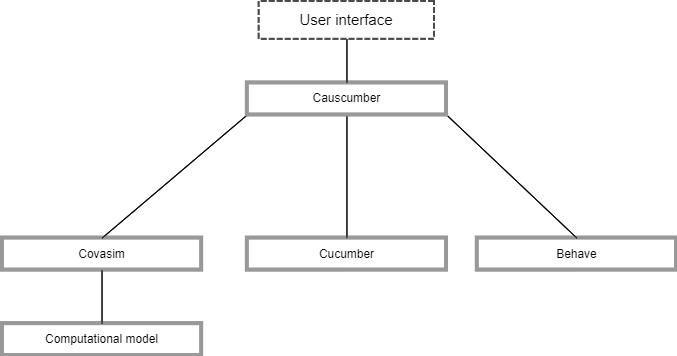
\includegraphics[width=13cm]{figures/Analysis.png}\\
	\caption{A diagram analysis for the system.}
	\label{fig:figure2}
\end{figure}
\section{Project Requirements}
Causcumber, is a tool that helps testers who aren’t trained in software to test a computational model, the goal of this project is to develop a tool that simplify the testing process of using Causcumber. In order to achieve this goal, first will need to understand how Causcumber work, Causcumber itself is a complex tool, it consist of codes from other API(Behave, Cucumber), and it also require to user follow various steps to test a model, this reverse engineering process need to be done in order to start working on the assist tool itself.\\*\\*
To test a model using Causcumber, user will need to define five separate files. First is the \textsl{dags} file, in this file user will need to define edges of the model, each edge consists of two parameter that are related to each other in some way, user will need to list out all the parameters in the model, and define the which parameter is related to which.\\*\\*
Second is the environment file, this one is a bit more complicated. User will need to setup multiple functions to initiate the testing data, execute the test itself, set the format of the produced result, and most importantly, the function to execute the tested model. This file require user to have a decent understanding in how to initiate data, and how to setup test using Causcumber. \\*\\*
The third files and fourth file are \textsl{dag\_steps} and \textsl{abstract}, these two files are python scripts for \textsl{Behave}. These files will need to define the step decorators for feature file, user will need to setup functions that can read the information in feature file and use the provided information to test the model and return the result. These two files will require user to understand how to setup decoder using the \textsl{Behave api}.\\*\\*
The fifth and final file is a feature file, in feature file user will need to set up test in the following order: 1. The background of the simulation (Value of parameter, etc.). 2. Is the edges user wish to test. 3. The scenario outline where user the define how will the change of a parameter should affect a group of parameters. 4. Scenario, where user define the expect behaviour of parameters if a parameter is altered. \\*\\*
As for the assisting tool, it should be able to assist tester in the process by reduce the need for tester interact with the coding part of testing directly. After that, this tool should be able to execute the feature file they have written, the system will examine the feature file and go through the computational model to check if the model performs as the test specifies. As a result, the system should produce a coherent result detailing the accuracy of the tested model. Thus, the systems need to accomplish the following:\\*
\\*
R1. As a user, I want this system to be easy to understand, when I use the system, I want to immediate know what I need to do to get the result I want.\\*
\\*
R2.As a user, I want to use the system to aid my testing process by reducing the need to code directly. \\*
\\*
R3. As a user, I want the system to go through the feature file I created and test the computational model with it.\\*
\\*
R4. As a user, I want the system to produce a result where I can know the accuracy of the computational model.\\*
\\*
Since Causcumber has been in development for a while, what this project aims to accomplish is adding more to this tool. Currently the state of Causcumber is capable of executing feature files to test models. And it is capable of returning a lot of useful information, but the information still requires some organization to make the result easier to read, also there isn’t a way to execute the testing system without using the terminal to execute the command. It also required testers to manually code every part of the test such as the DOT file that define the relation of the parameter, or the feature file that define the value and expected result. This makes testing with Causcumber still fairly complex, so there’s a need for a tool to assist people in operating the system. \\*\\*
To simplify and streamline the testing process, this tool should reduce the need for testers to interact with the code directly. Therefore, this tool for Causcumber should be able to accomplish the following:\\*
\\*
1. As a user, I want the result produced by the system to be clean and easy to understand, focusing on the important part.\\*
\\*
2. As a user, I want to have the ability to change to different scenarios, so I can test models under different settings.\\*
\\*
3. As a user, I want to have the ability to create new scenarios with essential files, so I can modify these files to test the model.\\*
\\*
4. As a user, I want to execute and interact with the system through a user interface.\\*
\\*
5. As a user, I want to have a more convenient way to create a feature file, to avoid any mistake during the creation of the feature file.\\*
\\*
6. As a user, I want to have a more simplify way to create a Dot file, to make the creating process less confusing. \\*
\\*

\section{Requirement analysis}
The first step of this project is to understand the workflow of Causcumber. To test a model, user will need to define several files to start the testing, in these files user will also need to define various aspect to test it. Organize and understand the purpose of these file will be the first step. Since the main theme for this project is simplify and ease of use, and therefore that’s what most of the requirements are focused on. For requirement R 1 – 4, the goal is to make the testing process as simple as possible, with a simplified testing process, people will be more willing to test their computational model with this tool. \\*\\*
To enhance the user experience for Causcumber, requirement 1, 2, 3 are aimed to achieve this. These requirements make using Causcumber to test computational models a more convenient experience. \\*\\
Since integrating the causal model testing can be difficult and confusing, requirements 4, 5, 6 are focused on simplifying this process, by making testing with Causcumber less code demanded, this should help mitigate a lot of errors and further simplify the testing process.
